\chapter{RESULTADOS PRELIMINARES}
\label{chap:resultados_discussao}

Este capítulo apresenta os resultados da prova de conceito realizada com os algoritmos desenvolvidos, tanto o modelo base quanto os modelos adaptados, com o intuito de compará-los aos objetivos traçados nesta dissertação. Os testes realizados buscam avaliar a eficiência dos algoritmos em diversas sob adaptações baseadas na intuição que a literatura ofereceu. O desempenho é analisado como também é discutido os resultados obtidos, este capítulo também oferece uma visão abrangente sobre os conjuntos de dados utilizados, destacando a relevância desses dados para a análise proposta.

%--------------------------------------------------------
\section{RESULTADOS ACDC}
\label{sec:resultados_acdc}

O conjunto de dados \gls{ACDC} foi a referência inicial, principalmente para a coleta dos resultados com o modelo base. Este conjunto de dados público já se encontra separado com $100$ exames para treino e $50$ para testes. A Figura \ref{fig:fig018} e \ref{fig:fig019} são exemplos respectivamente, de imagens de \gls{DCM} e \gls{HCM} capturadas na diástole com suas respectivas máscaras, lembrando que ambas representam cardiomiopatia hipertrófica. Na Figura \ref{fig:fig020} temos a imagem de coração em estado sem anomalia (\gls{NOR}) e sua respectiva máscara. As imagens demonstradas fazem parte do conjunto real de treinamento.

\begin{figure}[h!]
    \centering
    \caption{Captura Diastólica CMD}
    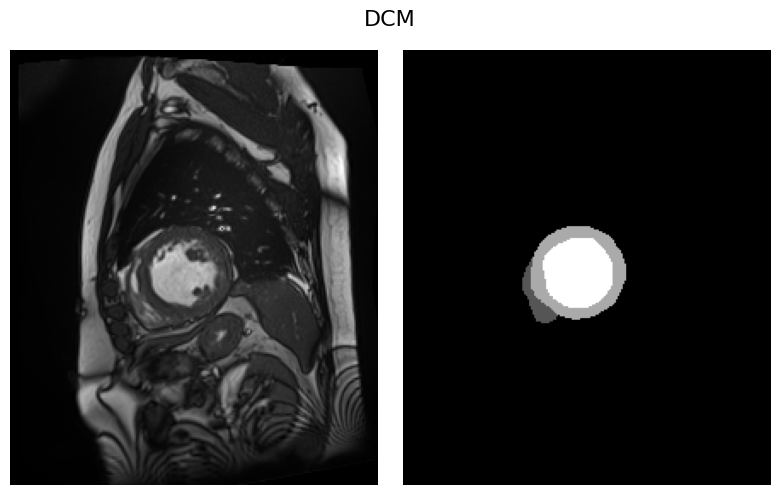
\includegraphics[width=0.65\textwidth]{figures/fig018.png}
    \caption*{Fonte: Autor}
    \label{fig:fig018}
\end{figure}

\begin{figure}[h!]
    \caption{Captura Diastólica de CMH}
    \centering
    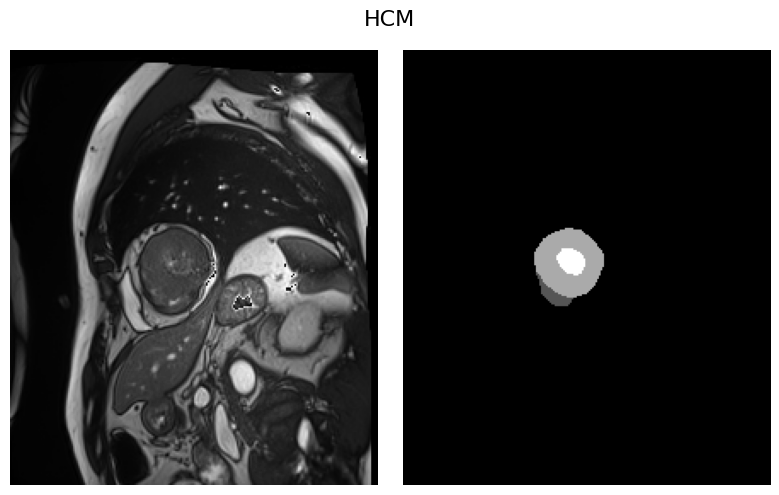
\includegraphics[width=0.65\textwidth]{figures/fig019.png}
    \caption*{Fonte: Autor}
    \label{fig:fig019}
\end{figure}

\begin{figure}[h!]
    \centering
    \caption{Captura Diastólica NOR}
    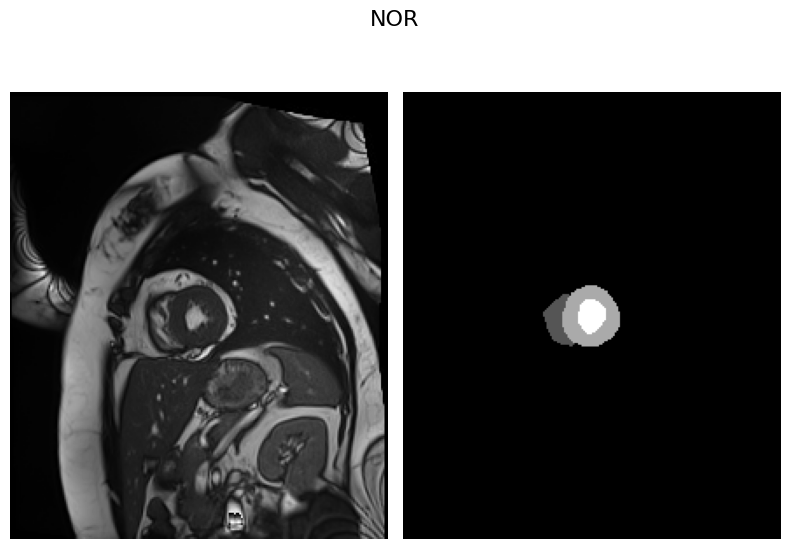
\includegraphics[width=0.65\textwidth]{figures/fig020.png}
    \caption*{Fonte: Autor}
    \label{fig:fig020}
\end{figure}

%--------------------------------------------------------
\subsection{RESULTADOS MODELO BASE}
\label{subsec:resultados_acdc_base}

Os resultados foram obtidos aplicando a metodologia previamente apresentada, foram extraídas as características radiômicas e profundas, após foi aplicado o \textit{F-Test} para seleção de características e o resultado concatenado na última dimensão, sendo $\textbf{EMBED}_{size} = 12$, o resultado é um vetor de características de $1\times24$. Em seguida, o modelo de autoatenção foi aplicado uma única vez conforma modelo original. Os hiperparâmetros utilizados são: taxa de aprendizado $\LR$, otimizador \gls{Adam}, tamanho de lote $\Batch$ e aproximadamente $\Epochs$ épocas. Por fim, é aplicada a função matemática sigmoide e definido o limite de $0,5$ para corte onde os valores acima deste limite são classificados como \gls{CMH} e os demais como normal. As métricas resultantes podem ser conferidas na Tabela \ref{tab:metrics}. A matriz de confusão é apresentada na Figura \ref{fig:fig016} e um gráfico ilustrando da \gls{ROC} é apresentado na Figura \ref{fig:fig017}.
\newline

\begin{table}[h!]
    \centering
    \caption{Métricas do Experimento - Modelo Base}
    \renewcommand{\arraystretch}{1} % default é 1 
    \begin{tabular}{|c|c|}
    \hline 
          \textbf{Métrica} & \textbf{Valor} \\ 
    \hline 
        Acurácia & 0.58 \\ 
    \hline 
        Precisão & 0.47 \\ 
    \hline 
        Revocação & 0.40 \\ 
    \hline 
        AUC & 0.55 \\ 
    \hline 
    \end{tabular} 
    \caption*{Fonte: Autor}
    \label{tab:metrics}
\end{table}

\begin{figure}[h!]
    \centering
    \caption{Matriz de Confusão -  Modelo Base}
    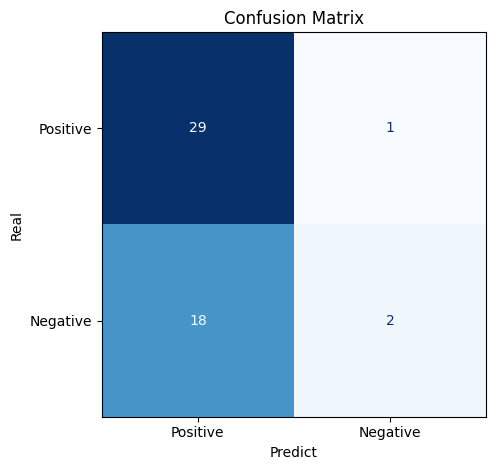
\includegraphics[width=0.55\textwidth]{figures/fig016.png}
    \caption*{Fonte: Autor}
    \label{fig:fig016}
\end{figure}

\begin{figure}[h!]
    \centering
    \caption{ROC}
    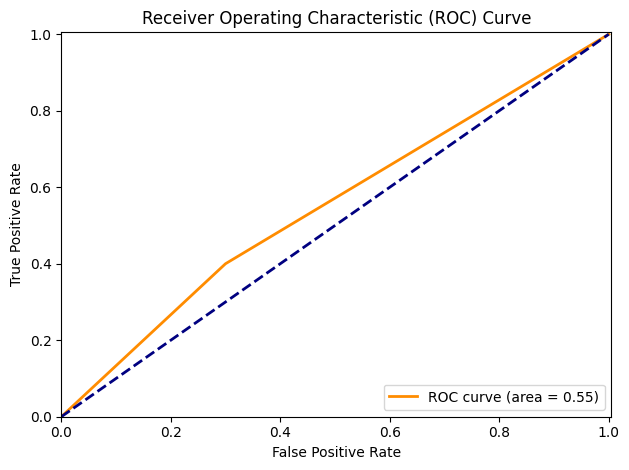
\includegraphics[width=0.75\textwidth]{figures/fig017.png}
    \caption*{Fonte: Autor}
    \label{fig:fig017}
\end{figure}


Para o registro dos resultados foi utilizado a ferramenta \textit{CometML}. O \textit{CometML} pode registrar, em tempo de execução, informações como erro por lote, erro por época, acurácia de validação, etc, podem ser armazenados enquanto o processo de treinamento é executado. Por fim métricas como acurácia e matriz de confusão podem ser geradas também.O serviço é acessado  por uma \gls{API} externa. As Figuras \ref{fig:fig028} e \ref{fig:fig029} demonstram respectivamente os painéis adaptáveis ao fim do treino e os valores armazenado de erro, acurácia, etc, coletados durante o treino. É possível notar que o modelo se sobre-ajusta nos dados de treino, predizendo corretamente todos os valores porém, nos dados de treino,  a assertividade cai drasticamente para $0,58$. Também é possível notar que após $2500$ passos no treinamento, o erro estabiliza e o demais processamento não necessariamente se faria necessário.

\begin{figure}[h!]
    \centering
    \caption{Painéis Adaptáveis - \textit{CometML}}
    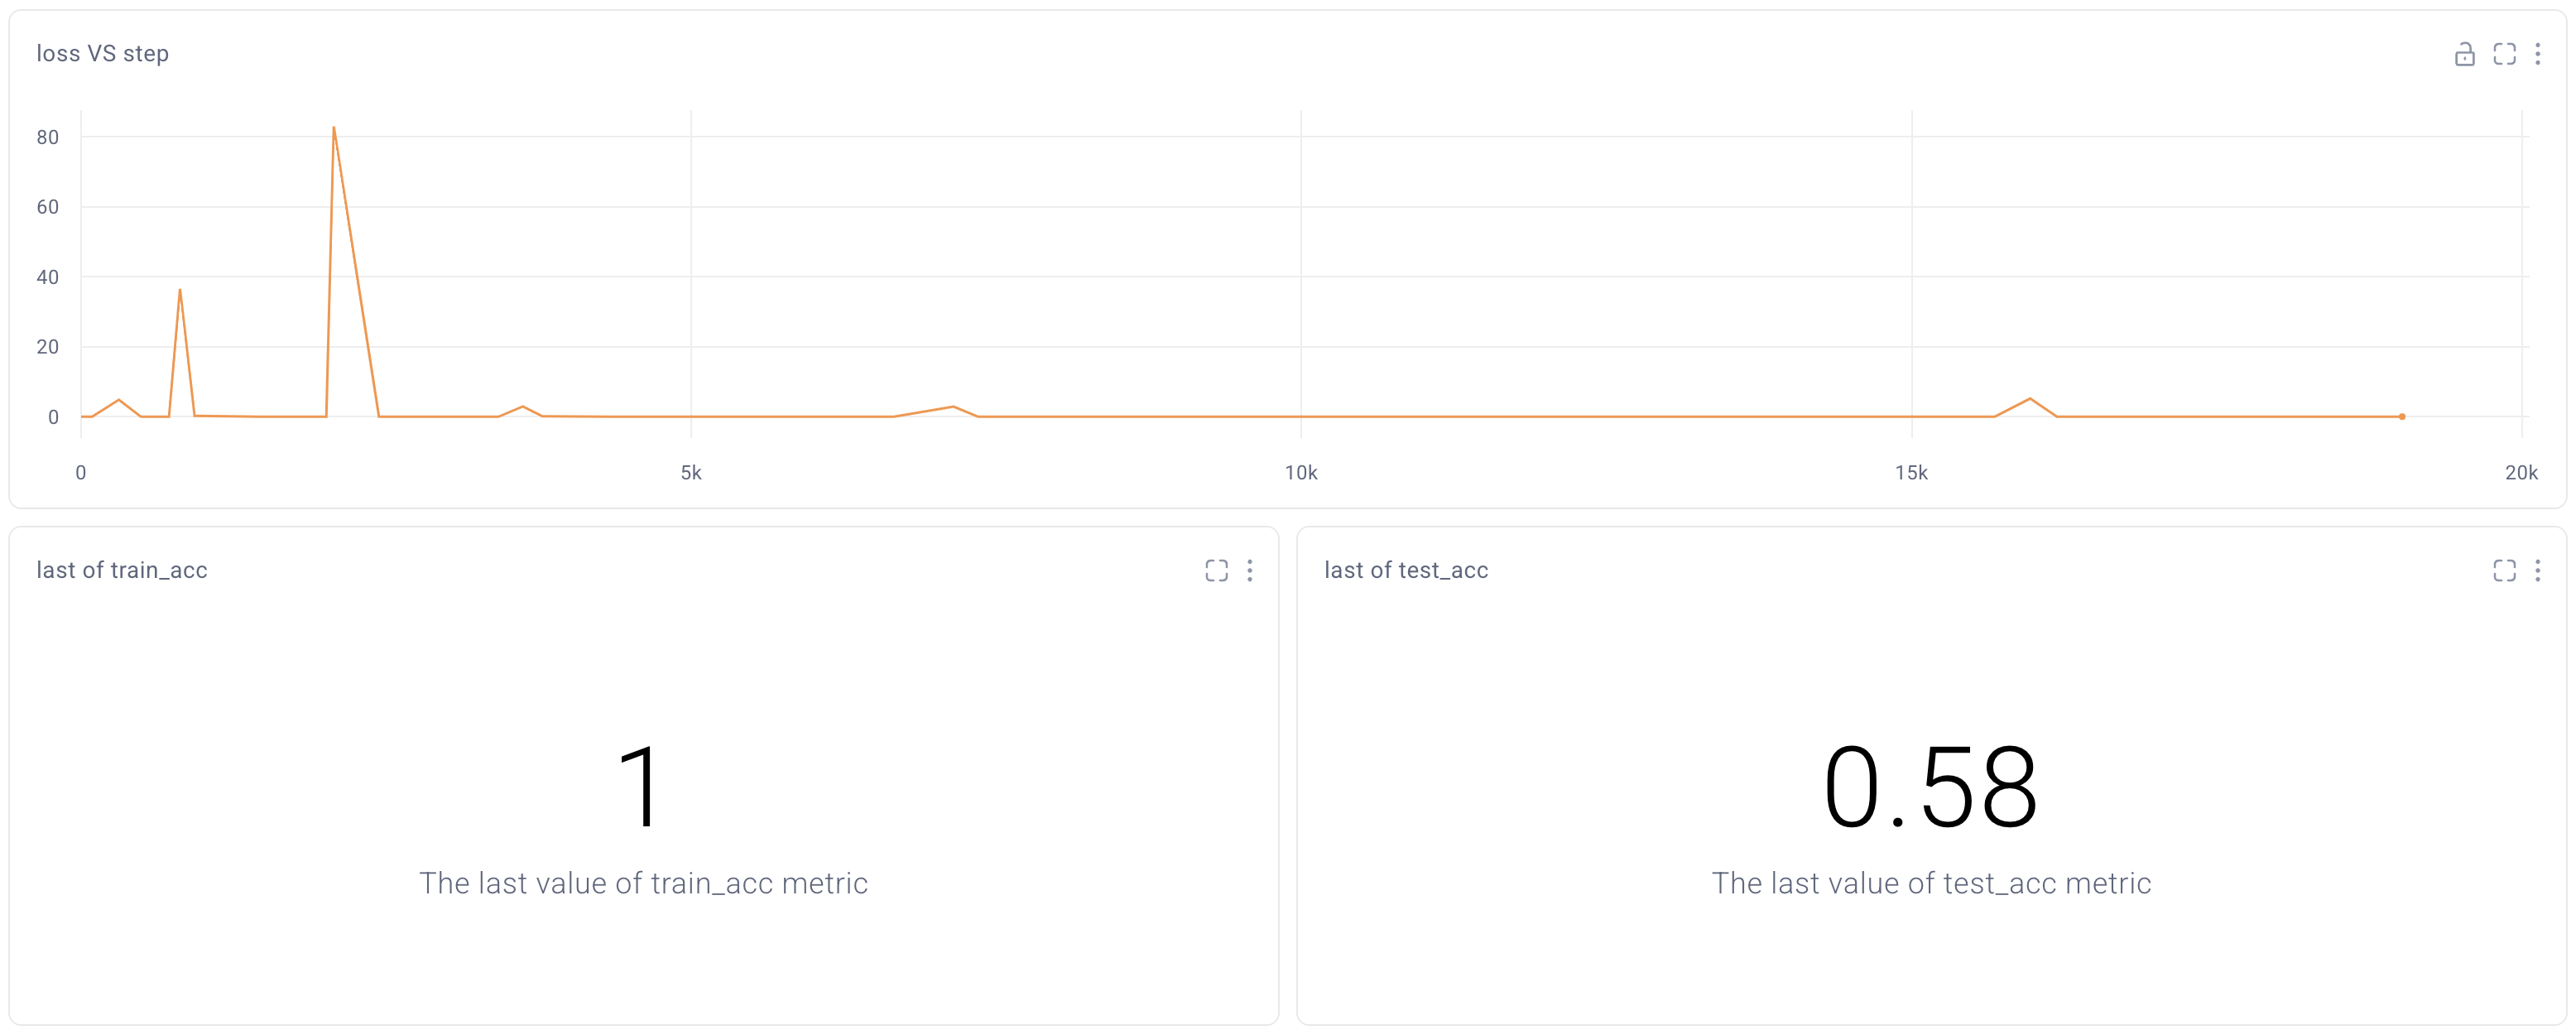
\includegraphics[width=1\textwidth]{figures/fig028.png}
    \caption*{Fonte: Autor}
    \label{fig:fig028}
\end{figure}


\begin{figure}[h!]
    \centering
    \caption{Valores Coletados no Treino - \textit{CometML}}
    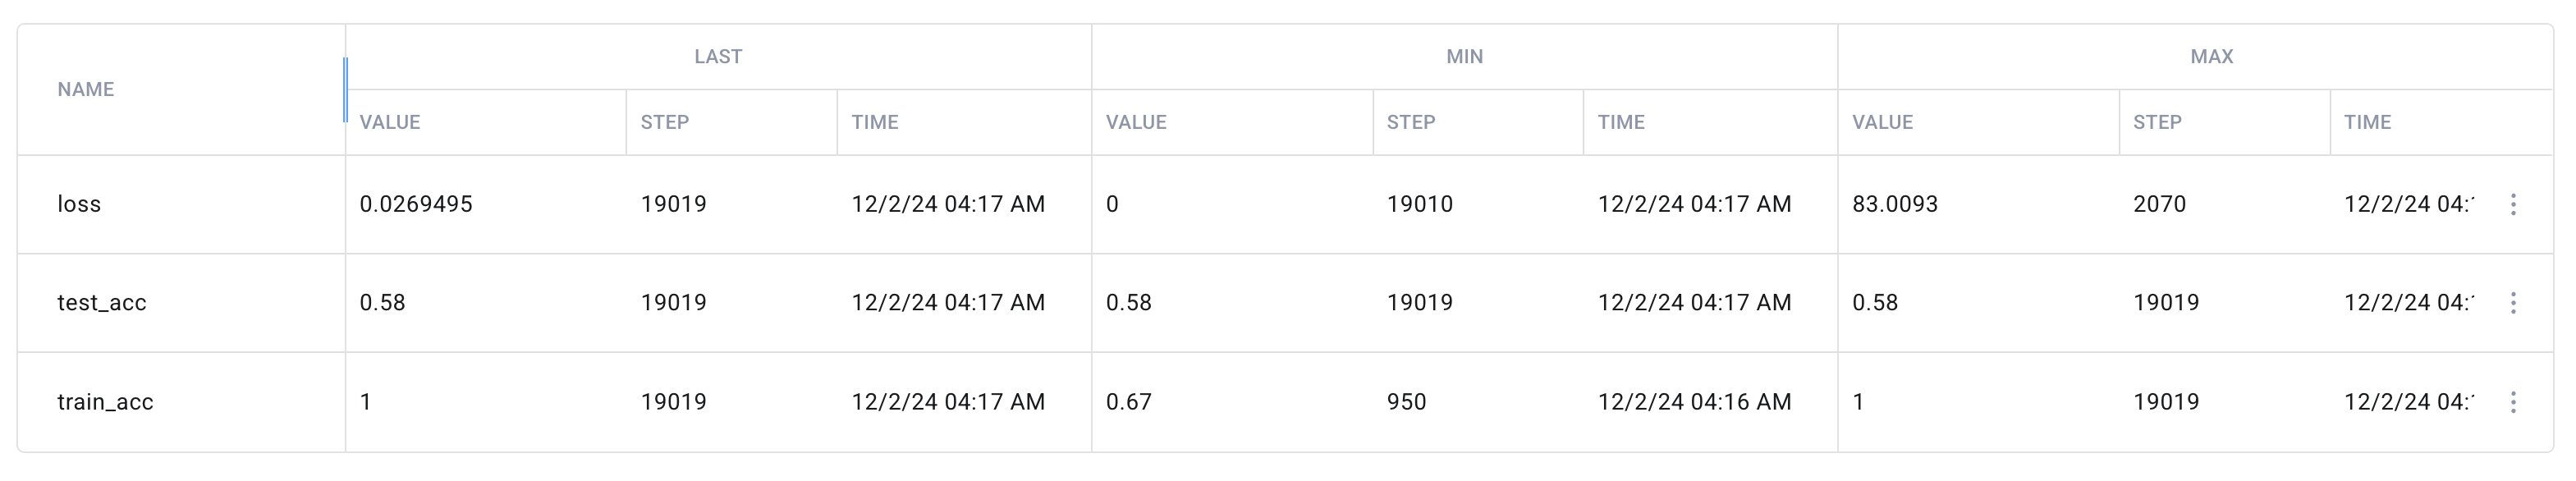
\includegraphics[width=1\textwidth]{figures/fig029.png}
    \caption*{Fonte: Autor}
    \label{fig:fig029}
\end{figure}


%--------------------------------------------------------
\subsection{Resultados dos Modelos Adaptados - ACDC}
\label{subsec:resultados_acdc_adaptado}

Para as versões adaptadas, buscou mudar os hiperparâmetros e até mesmo a arquitetura do modelo com o intuito comparar os resultados com a versão base. Os primeiros experimentos foram aplicados mudando o $\textbf{EMBED}_{size}$ para outros valores, também foi aplicado $N$ vezes o bloco de autoatenção ao invés de uma única vez. Os valores de $N$ utilizados foram $[1, 2, 4, 6]$. Estas mudanças não mudaram a estrutura da arquitetura fazendo com que o módulo autoatenção seja executado $N$ vezes conforme trabalho de \cite{vaswaniAttentionAllYou2023} e pode ser visualizada na Figura \ref{fig:fig030}.

\begin{figure}[h!]
    \centering
    \caption{Recorrência do Módulo de Autoatenção}
    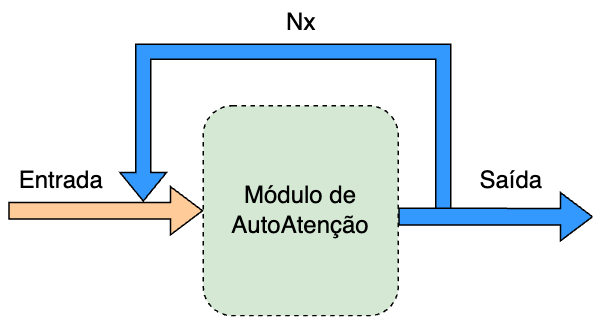
\includegraphics[width=0.7\textwidth]{figures/fig030.png}
    \caption*{Fonte: Autor}
    \label{fig:fig030}
\end{figure}

Também foi introduzido, nas versões adaptadas, um módulo convolucional, que antecede o módulo de auto atenção. Este módulo convolucional contém uma camada convolucional 1D, um bloco \gls{SE} e por fim outro bloco convolucional 1D. Dado o fato de termos três vetores de características, com a adição da máscara, identificar relações intrínsecas entre estes vetores previamente ao módulo de autoatenção foi um dos experimentos. A concatenação agora da na primei dimensão faz cada vetor de característica ser interpretado como um canal. Uma primeira camada de convolução 1D aumenta o número de canais para 16, ou seja, 16 filtros são aplicado para extração de informação espacial. O bloco \gls{SE} representa uma camada de atenção seletiva que dá importância aos canais mais importantes. Ela identifica a relevância de cada canal e finaliza escalando os canais na entrada original com um valor escalar otimizado em tempo de treinamento, detalhes podem ser vistos na Figura \ref{fig:fig031}. O bloco \gls{SE} neste projeto é adaptado para ser 1D, diferente do trabalho original que visa sua aplicação em modelos de visão computacional já consolidados. O valor de $r$ no bloco \gls{SE} ficou fixo em $16$, os autores do trabalho original fazem testes empíricos e confirmam que o valor de $16$ é que traz melhores resultados.

\begin{figure}[h!]
    \centering
    \caption{Composição Bloco SE}
    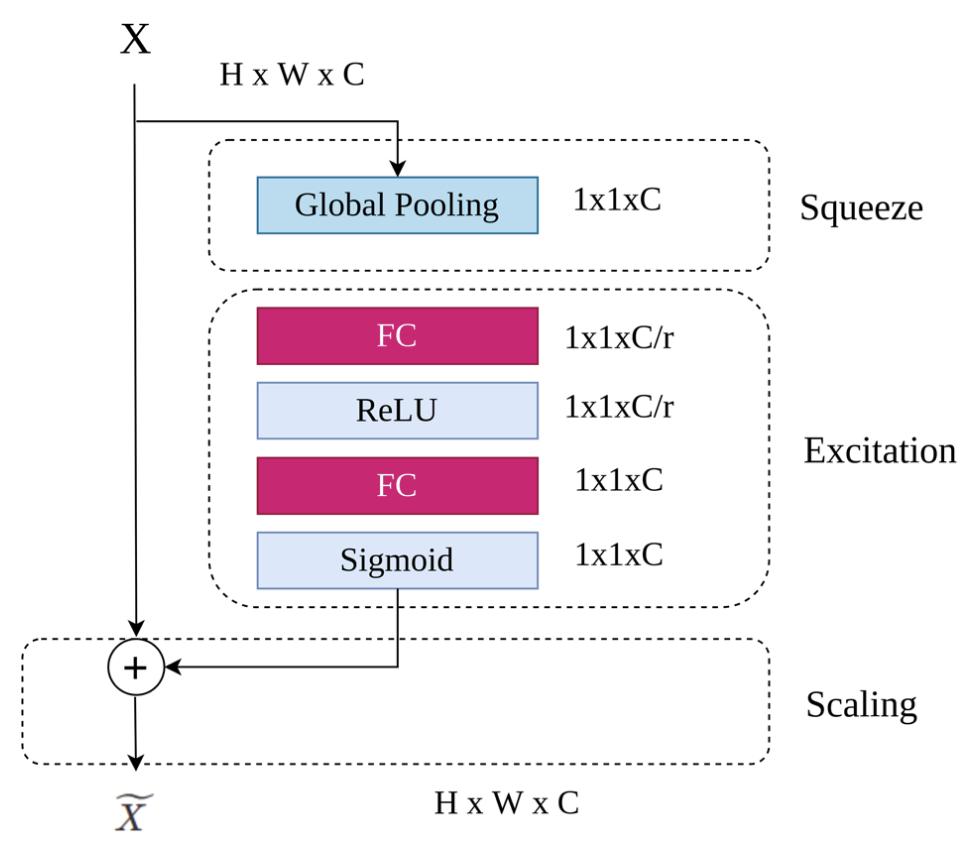
\includegraphics[width=0.7\textwidth]{figures/fig031.png}
    \caption*{Fonte: Adaptado de \cite{lafraxoSEDARUnetSqueezeexcitationDilated2024}}
    \label{fig:fig031}
\end{figure}

As tabelas que seguem demonstram respectivamente um conjuntos de experimentos na versão original adaptada na Tabela \ref{tab:metrics_orig}, um versão adicionando as máscaras como terceiro vetor de características na Tabela \ref{tab:metrics_orig_mask} e, por fim, a versão que adiciona os blocos convolucionais e \gls{SE} na Tabela \ref{tab:metrics_se}. Alguns pontos são notados no experimento, o treinamento quase sempre sofre sobre-ajuste ficando muito próximo de 100\% de assertividade, isso pode se dar ao fato de haver poucos exemplares para treinamento. Outro ponto notado é que quanto maior o tamanho do vetor de características (Emb) melhor costuma ser o resultado. Quantidades maiores de blocos de autoatenção (N\_Attn) costumam trazer melhores, exceto no caso em que são configurados em $6$ pois os melhores resultados são quando configurados em $4$. Isso se deve ao fato de trazer excesso de complexidade ao modelo que não exige dado ao fato de um conjunto de dados limitado. Os melhores resultados são conferidos nas versões que adicionam o bloco \gls{SE}, se verificando o melhor experimento que alcançou $80\%$ de assertividade em azul. A visualização dos modelos com bloco \gls{SE}, armazenados no \textit{CometML} é visto na Figura


\begin{table}[htbp]
\centering
\caption{Tabela de Métricas - Adaptação do Modelo Original}
\begin{tabular}{lcccccc}
\toprule
\textbf{Emb} & \textbf{N\_Attn} & \textbf{Acc} & \textbf{Precision} & \textbf{Recall} & \textbf{F1} & \textbf{AUC} \\
\midrule
\textcolor{orange}{24} & \textcolor{orange}{1} & \textcolor{orange}{0.58} & \textcolor{orange}{0.47} & \textcolor{orange}{0.45} & \textcolor{orange}{0.46} & \textcolor{orange}{0.55} \\
24 & 2 & 0.58 & 0.48 & 0.60 & 0.53 & 0.58 \\
24 & 4 & 0.54 & 0.44 & 0.55 & 0.49 & 0.54 \\
24 & 6 & 0.50 & 0.41 & 0.55 & 0.47 & 0.51 \\
\hline
48 & 1 & 0.62 & 0.52 & 0.55 & 0.54 & 0.61 \\
48 & 2 & 0.64 & 0.54 & 0.65 & 0.59 & 0.64 \\
48 & 4 & 0.66 & 0.56 & 0.70 & 0.62 & 0.67 \\
48 & 6 & 0.64 & 0.54 & 0.70 & 0.61 & 0.65 \\
\hline
64 & 1 & 0.62 & 0.52 & 0.65 & 0.58 & 0.62 \\
64 & 2 & 0.64 & 0.54 & 0.70 & 0.61 & 0.65 \\
64 & 4 & 0.66 & 0.57 & 0.65 & 0.60 & 0.66 \\
64 & 6 & 0.64 & 0.54 & 0.65 & 0.59 & 0.64 \\
\bottomrule
\end{tabular}
\caption*{Fonte: Autor}
\label{tab:metrics_orig}
\end{table}


\begin{table}[htbp]
\centering
\caption{Tabela de Métricas - Adaptação do Modelo Original Com Máscaras}
\begin{tabular}{lcccccc}
\toprule
\textbf{Emb} & \textbf{N\_Attn} & \textbf{Acc} & \textbf{Precision} & \textbf{Recall} & \textbf{F1} & \textbf{AUC} \\
\midrule
24 & 1 & 0.44 & 0.35 & 0.45 & 0.39 & 0.44 \\
24 & 2 & 0.46 & 0.38 & 0.55 & 0.45 & 0.48 \\
24 & 4 & 0.48 & 0.36 & 0.40 & 0.38 & 0.47 \\
24 & 6 & 0.48 & 0.38 & 0.45 & 0.41 & 0.47 \\
\hline
48 & 1 & 0.52 & 0.44 & 0.70 & 0.54 & 0.55 \\
48 & 2 & 0.58 & 0.48 & 0.55 & 0.51 & 0.57 \\
48 & 4 & 0.62 & 0.52 & 0.60 & 0.56 & 0.62 \\
48 & 6 & 0.60 & 0.50 & 0.50 & 0.50 & 0.58 \\
\hline
64 & 1 & 0.58 & 0.48 & 0.60 & 0.53 & 0.58 \\
64 & 2 & 0.56 & 0.45 & 0.50 & 0.48 & 0.55 \\
64 & 4 & 0.64 & 0.54 & 0.65 & 0.59 & 0.64 \\
64 & 6 & 0.62 & 0.53 & 0.45 & 0.49 & 0.59 \\
\bottomrule
\end{tabular}
\caption*{Fonte: Autor}
\label{tab:metrics_orig_mask}
\end{table}


\begin{table}[htbp]
\centering
\caption{Tabela de Métricas - Adaptação Adicionando Blocos Conv. e SE}
\begin{tabular}{lcccccc}
\toprule
\textbf{Emb} & \textbf{N\_Attn} & \textbf{Acc} & \textbf{Precision} & \textbf{Recall} & \textbf{F1} & \textbf{AUC} \\
\midrule
24 & 1 & 0.66 & 0.56 & 0.70 & 0.62 & 0.67 \\
24 & 2 & 0.68 & 0.58 & 0.75 & 0.65 & 0.69 \\
24 & 4 & 0.70 & 0.59 & 0.80 & 0.68 & 0.72 \\
24 & 6 & 0.68 & 0.59 & 0.65 & 0.62 & 0.67 \\
\hline
48 & 1 & 0.70 & 0.58 & 0.90 & 0.71 & 0.73 \\
48 & 2 & 0.70 & 0.62 & 0.65 & 0.63 & 0.69 \\
48 & 4 & 0.74 & 0.65 & 0.75 & 0.70 & 0.74 \\
48 & 6 & 0.70 & 0.60 & 0.75 & 0.67 & 0.71 \\
\hline
64 & 1 & 0.64 & 0.54 & 0.65 & 0.59 & 0.64 \\
64 & 2 & 0.72 & 0.64 & 0.70 & 0.67 & 0.72 \\
\textcolor{blue}{64} & \textcolor{blue}{4} & \textcolor{blue}{0.80} & \textcolor{blue}{0.73} & \textcolor{blue}{0.80} & \textcolor{blue}{0.76} & \textcolor{blue}{0.80} \\
64 & 6 & 0.76 & 0.65 & 0.85 & 0.74 & 0.77 \\
\bottomrule
\end{tabular}
\caption*{Fonte: Autor}
\label{tab:metrics_se}
\end{table}


\begin{figure}[h!]
    \centering
    \caption{Visão dos Modelos c/ Bloco SE - \textit{CometML}}
    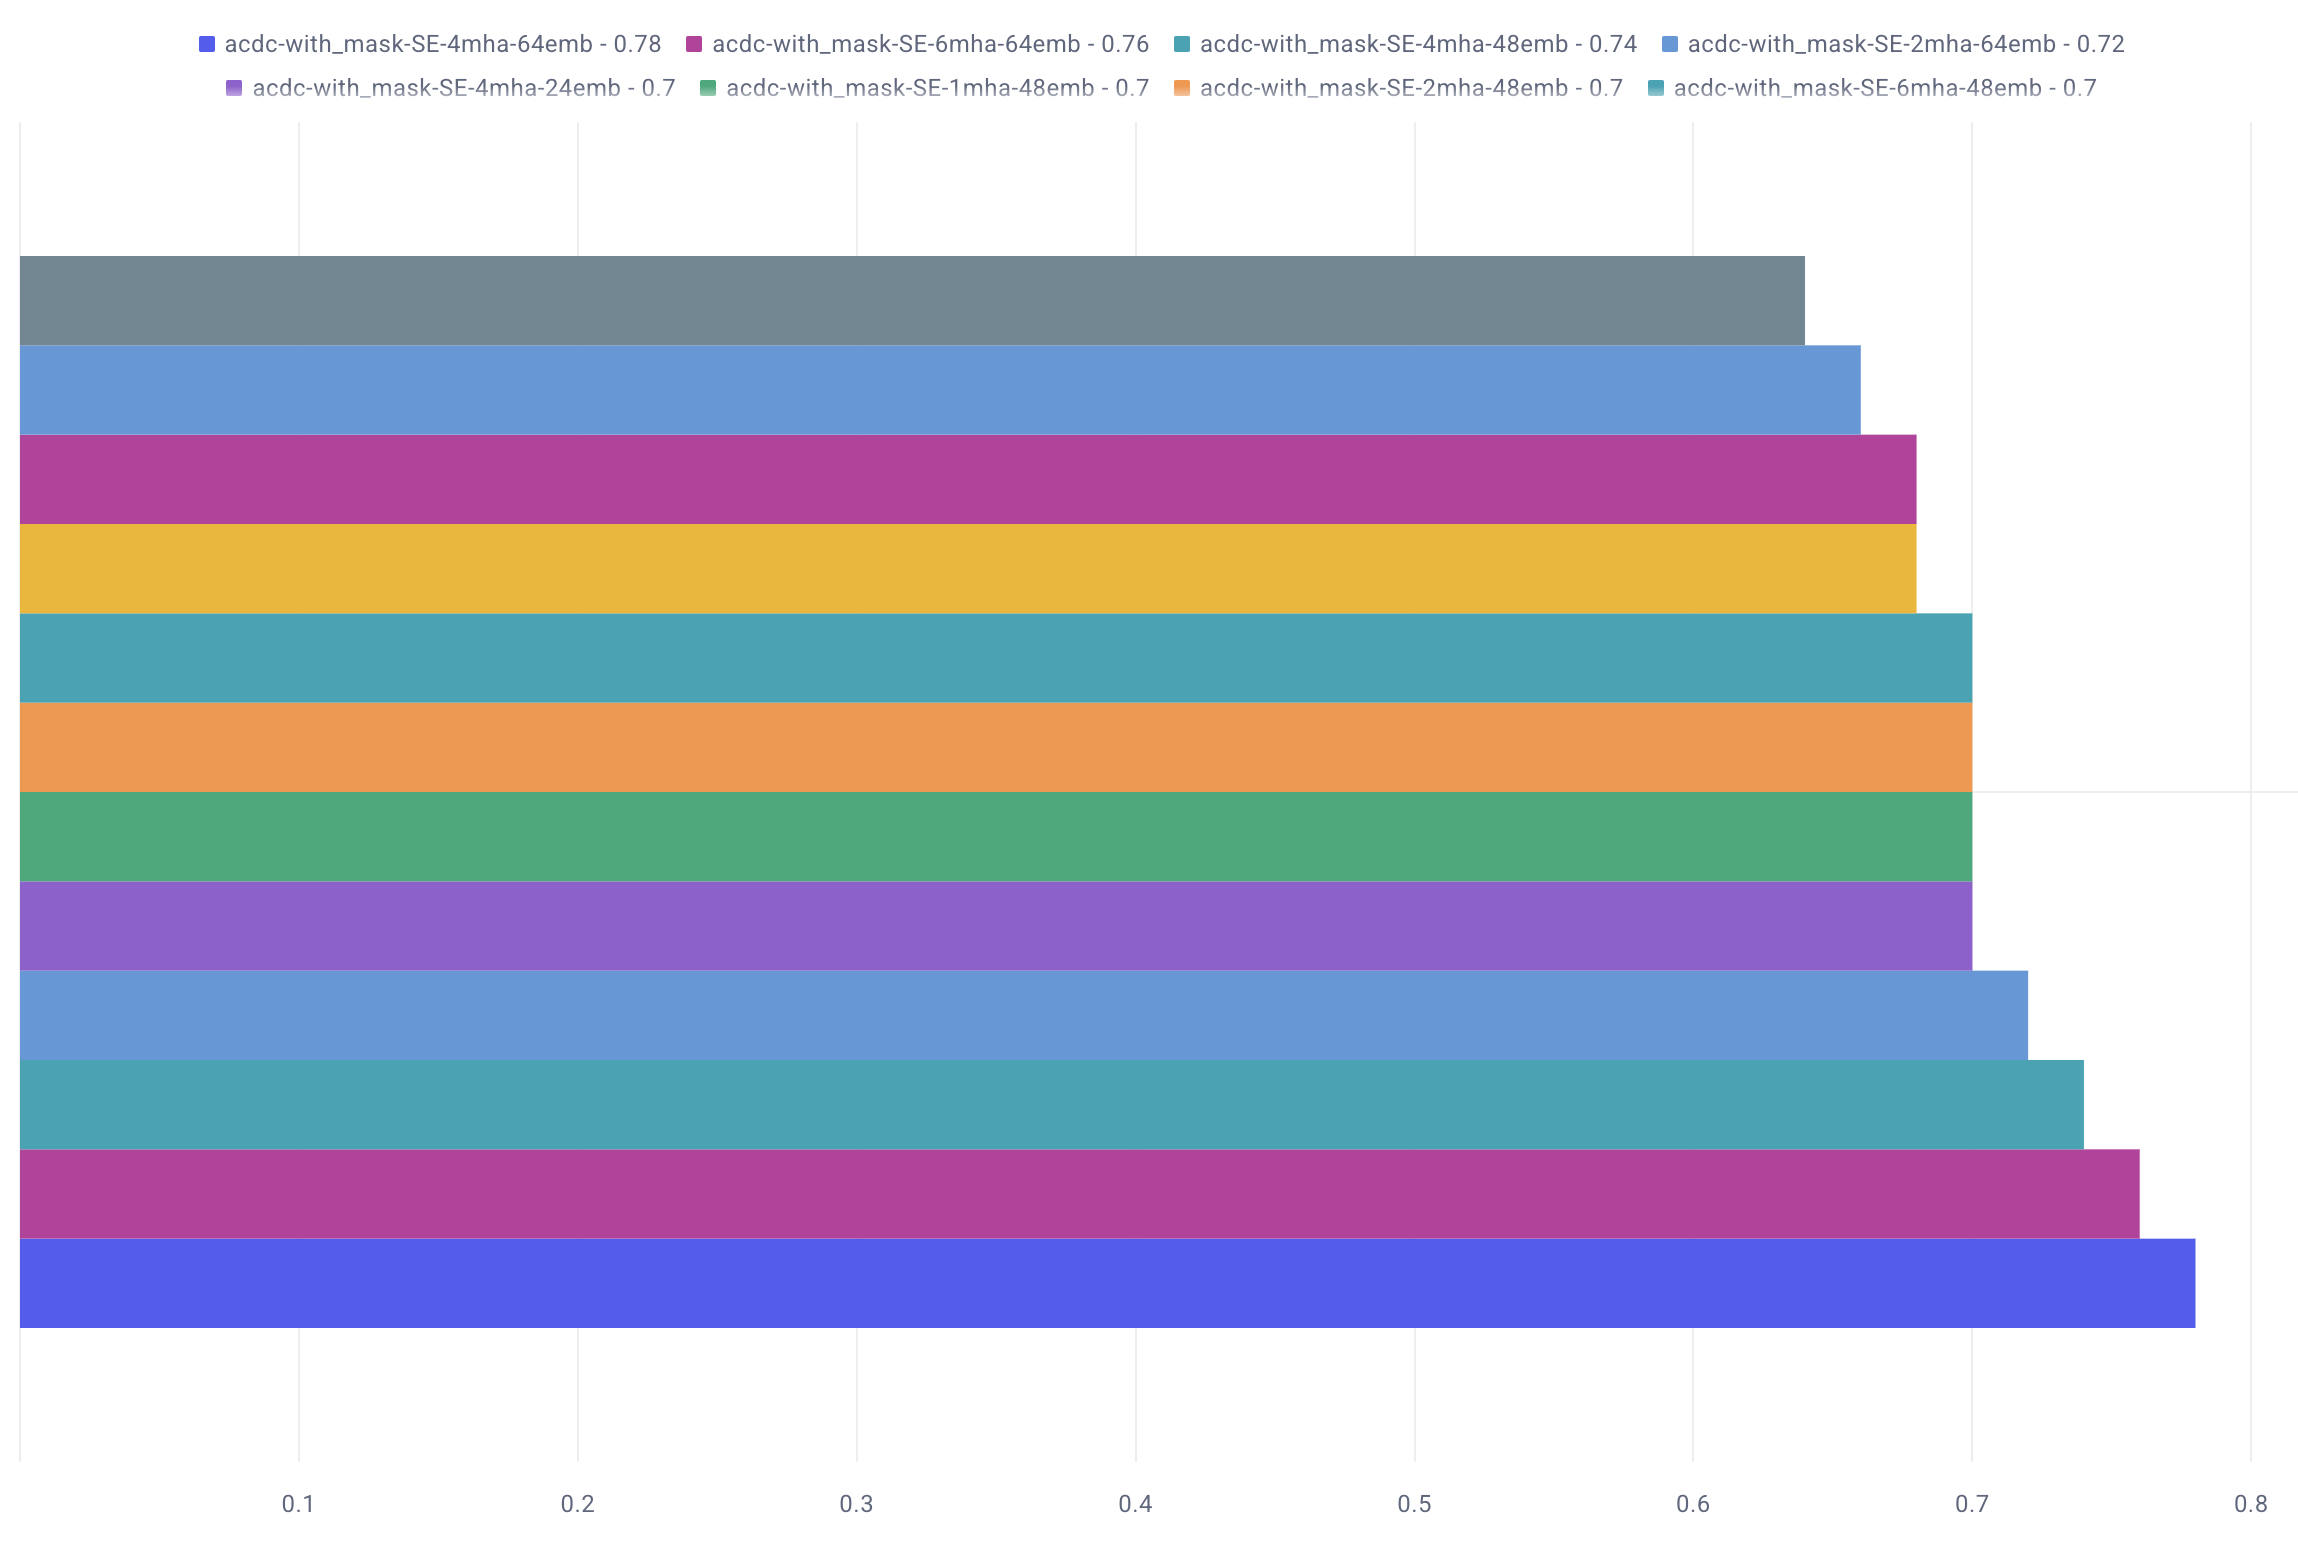
\includegraphics[width=1\textwidth]{figures/fig032.png}
    \caption*{Fonte: Autor}
    \label{fig:fig032}
\end{figure}

%--------------------------------------------------------
\subsection{Resultados dos Modelos Adaptados - \textit{SunnyBrook}}
\label{subsec:resultados_sunny_adaptado}

Os experimentos no conjunto de dados \textit{SunnyBrook} foram praticamente igualis aos aplicados ao conjunto de dados \gls{ACDC}. Houver uma etapa extra no pré-processamento, para gerar as máscaras das imagens de RM precisa-se interpolar os valores de um arquivo de texto que vem anexo com os dados. A máscara também é composta apenas pela região de interesse contanto apenas valores 0 e 1.

%--------------------------------------------------------
\section{Considerações Finais do Capítulo} 
\label{sec:cap6_consideracoes_finais}

Os resultados obtidos, aplicando a arquitetura proposta por \citeonline{aiSelfAttentionBasedFusion2023} com modificações na quantidade de características utilizadas e aplicado em imagens de \gls{RMC} para identificação de cardiomiopatias, em contraste com o trabalho mencionado que foi aplicado à identificação de câncer no pulmão, obteve resultados menos relevantes que o original. Isto indica que há espaço para exploração e melhorias a serem proposta para o âmbito de cardiomiopatia. Algumas, abordagens ainda são tidas em vista como manipular o seletor de características e a sua quantidade, testar novos hiperparâmetros para os modelos, ao invés de ter um único módulo de autoatenção, aplicar vários em cascata, etc.

